\chapter{Audio Signal Processing and Inverse Problem}\label{ch:processing}
\openepigraph{Sound, a certain movement of air.}{Aristotele, De Anima II.8 420b12}
\vspace{-2.5em}
\newthought{Synopsis} Let us now move from the physical domain to discrete time
signal processing
\blindtext[1]
Notation and definition are based on \cite{gannot2017consolidated}.

\section{Signal Model and Definitions}
\marginpar{
    \footnotesize
    In this section and in the rest of the dissertation,
    we adopt the following general notations defined in~\cpageref{ch:notation}
    and introduced by \citeonly{gannot2017consolidated}.
}
In this thesis, an \textit{auditory} scene consists in sound \textit{sources}, \textit{microphones} deployed in a room.
The signals are emitted by sources and they are observed, received or recorded by microphones.
A set of microphones is called a microphone \textit{array} and its signal are called \textit{channels}.

Let us assume the observed signal has $\numMics$ \textit{channels} indexed by $\idxMic \in \kbrace{1,\dots,\numMics}$.
A \textit{single-channel} signal ($\numMics = 1$) is represented by the scalar $\mic(t) \in \bbR$,
while a \textit{multichannel} ($\numMics >   1$) is represented by the vector
$\mics(t) = \ktranspose{\klist{\mic_1(t), \dots, \mic_{\numMics}(t)}} \in \bbR^{\numMics \times 1}$.
The $\idxMic$-th microphone have a well defined position in the space which is denoted with $\positionMicrophone_\idxMic$.
\\Furthermore, let assume that there are $\numSrcs$ sources indexed by $\idxSrc \in \numSrcs$.
Sources can be of two types:
\begin{description}
    \item[Point sources] are emitted by a single and well-defined point in the space $\positionSource_\idxSrc$ and their signal is single channel.
    Point sources are for instance human speakers or the sound emitted by a loudspeaker.
    \item[Diffuse sources] refers for instance to wind, traffic noise, or large musical instruments, which emit sound in a large region of space.
    Their sound cannot be associate to a punctual source, but rather a distributed (infinite) collection of them.
\end{description}

\newthought{The Mixing Process} leading to the observed signal can be
using by means of an intermediate representation~\cite{sturmel2012linear}:
\begin{center}
    \textit{The \emph{source spatial images}, or \emph{images},  $\img_{\idxMic\idxSrc}(t)$ describes the contribution
    of the source $\idxSrc$ to the microphone $\idxMic$ by means of a spatialization
    operation\sidenote{\eg/ the propagation from the point source to the microphone including reverberation}}.
\end{center}
Being $\spat_\idxSrc(\cdot)$ a possibly nonlinear spatialization operation, the spatial images
$\imgs_\idxSrc(t) = \ktranspose{\klist{\img_{1\idxSrc}(t), \dots, \img_{\numMics\idxSrc}(t)}}$ with respect to the $\numMics$ reads
\begin{equation}
    \imgs_\idxSrc(t) = \kbracket{\spat_\idxSrc(\src_\idxSrc)}(t)
    .
\end{equation}
In second stage, the images of all (point and diffuse) sources are added together and passed through a possibly
nonlinear \textit{post-mixing} operation $\master(\cdot)$ to obtain the mixture signal $\mics(t)$
\begin{equation}
    \mics(t) = \kbracket{ \master\kparen{
                    \sum_{\idxSrc=1}^{\numSrcs} \imgs_\idxSrc
                    }}(t)
\end{equation}
\marginpar{
    \footnotesize
    In the field of music productions,
    $\spat_\idxSrc(\cdot)$ and $\master(\cdot)$ may be identify rispectively with the \textit{mixing} and \textit{mastering} process.
}
\begin{figure}[t]
    \centering
    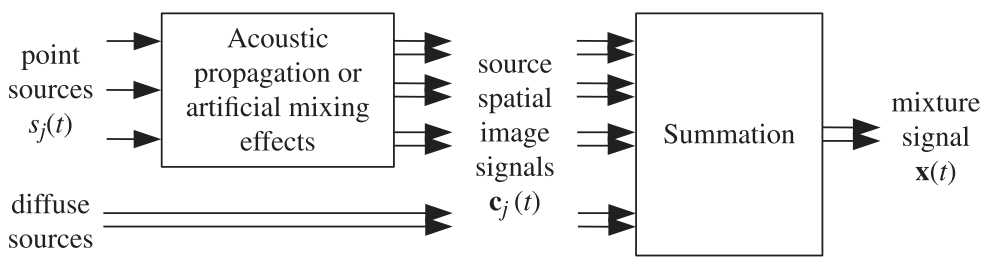
\includegraphics[width=\linewidth]{processing/mixing_process.png}
    \caption{General mixing process,
    illustrated in the case of $\numSrcs = 4$ sources,
    including three point sources and one diffuse source, and $\numMics = 2$ channels.}
    \label{fig:processing:mixing}
\end{figure}
\textsc{In Room Acoustics, the mixing process} is due to the propagation of sound in the auditory scene.
As discussed in~\cref{ch:acoustics:sec:wave}, this process is linear (and time invariant provided a static scenario).
In this case, the spatialization operation $\spat_\idxSrc(\cdot)$ is expressed by
collection of convolution with \RIR/ $h_{\idxMic\idxSrc}$
from source $\idxSrc$ to microphone $\idxMic$ and the post-mixing operation $\master(\cdot)$ reduces to the identity:
\begin{align}
    \img_{\idxMic\idxSrc}(t) &=  \kparen{h_{\idxMic\idxSrc} \conv \src_\idxSrc} (t) \\
    \imgs_\idxSrc(t) &=  \ktranspose{\klist{\img_{1\idxSrc}(t), \dots, \img_{\numMics\idxSrc}(t)}}\\
    \mics(t)         &= \sum_{\idxSrc=1}^{\numSrcs} \imgs_\idxSrc(t)
\end{align}
where $\conv$ is the linear convolution operator.
% \sum_{\tau=-\infty}^{+\infty} \bsh_\idxSrc(\tau) s_\idxSrc(t - \tau)
%
Target noise

\subsection{Time-Frequency Analysis and Synthesis}

\subsection{Artificial Mixtures}

\subsection{Impulse Response Models}
\newthoughtpar{Acoustic and Room Impulse Response}

\newthoughtpar{Acoustic and Room Transfer Functions}

\newthoughtpar{Steering Vectors}

\newthoughtpar{Relative Transfer Functions}

\newthoughtpar{Full-Rank Covariance Models}

%%%%%%%%%%%%%%%%%%%%%%%%%%%%%%%%
\section{Audio Inverse Problems}
\newthoughtpar{Forward vs Inverse Problem}

\subsection{General Processing Scheme}
General Processing Pipeline

\subsection{Some Audio Inverse Problems}
\begin{enumerate}
    \item sound source separation and enhancements
    \item sound source localization
    \item microphones calibration
    \item channel estimation
    \item room geometry estimation
    \item acoustic echo estimation
\end{enumerate}
\newthoughtpar{Evaluation}

%%%%%%%%%%%%%%%%%%%%%%%%%%%%%%%%
\section{Taxonomy through dichotomies}
%% acoustics %%
\newthoughtpar{Single-Channel vs. Multichannel}
\newthoughtpar{Point vs. Diffuse Sources}
\newthoughtpar{Directonal vs. Onmidirectional Recordings}
\newthoughtpar{Diffuse vs. Measurements Noise}
%% processing %%
\newthoughtpar{Natural vs. Artificial Mixtures}
%% pipeline %%
\newthoughtpar{Problem vs. Model}
\newthoughtpar{Synthesis vs. Abstaction}
%% problems %%
\newthoughtpar{Separation vs. Enhancement}
%% models %%
\newthoughtpar{end2end vs. 2step}
end2end: from data to (feature to) target
\\2-step: (from data to features) + features to target

\newthoughtpar{Knowledge-based vs. Learning-based}
\begin{itemize}
    \item Bottom-up vs Top-down information processing
    \item Knowledge-based: specialized signal processing and mathematical algorithms informed by knowledge;
    \item Learning-based: machine learning usually trained in supervised fashion.
\end{itemize}

\newthoughtpar{Supervised vs. Unsupervised}
\newthoughtpar{Machine Learning vs. Deep Learning}